\documentclass[conference]{IEEEtran}
\IEEEoverridecommandlockouts
\usepackage{cite}
\usepackage{amsmath,amssymb,amsfonts}
\usepackage{algorithmic}
\usepackage{graphicx}
\usepackage{textcomp}
\usepackage{xcolor}
\usepackage{tikz}
\usetikzlibrary{shapes.geometric, arrows.meta, positioning, fit, backgrounds, calc, shadows}
\usepackage{array}
\usepackage{booktabs}
\usepackage{multirow}
\usepackage{tabularx}
\usepackage{url}
\usepackage{hyperref}

\def\BibTeX{{\rm B\kern-.05em{\sc i\kern-.025em b}\kern-.08em
    T\kern-.1667em\lower.7ex\hbox{E}\kern-.125emX}}

\begin{document}

\title{SheGuard: Resilient Offline-First Mobile Safety Architecture with Deterministic Multimodal Fusion, Cryptographic Evidence Sealing, and Peer Relay Escalation}

\author{\IEEEauthorblockN{Zainulabideen Pawle}
\IEEEauthorblockA{\textit{Department of Computer Engineering} \\
\textit{Anjuman-I-Islam's Kalsekar Technical Campus (AIKTC)}\\
Panvel, Navi Mumbai, India \\
zainpawle19@gmail.com}
\and
\IEEEauthorblockN{Sarah Ansari}
\IEEEauthorblockA{\textit{Department of Computer Engineering} \\
\textit{Anjuman-I-Islam's Kalsekar Technical Campus (AIKTC)}\\
Panvel, Navi Mumbai, India \\
ansarisarah463@gmail.com}
}

\maketitle

\begin{abstract}
Many mobile safety applications depend on manual SOS activation, continuous network connectivity, or a single detection modality, limiting their reliability when a user cannot operate a device or network access is unavailable. This paper presents \textbf{SheGuard}, an offline-first Android safety companion that combines on-device acoustic, keyword, and motion sensing with deterministic incident management. The system uses distress-sound classification, configurable speech-command detection, and accelerometer-based motion analysis. These signals are evaluated by a rule-based fusion engine before entering an auditable incident state machine with a bounded user-confirmation interval and default-to-escalate semantics. Following incident confirmation, SheGuard attempts emergency delivery through peer-to-peer relays over Bluetooth Low Energy or Wi-Fi Direct, with cellular-only Short Message Service fallback when relay peers or data connectivity are unavailable. In parallel, the system captures incident evidence locally, protects it using per-incident authenticated encryption, and preserves its integrity through SHA-256 hashing, Merkle-tree sealing, and Android Keystore-backed signing. A separate human-in-the-loop assistance layer supports incident summarization and First Information Report drafting without participating in emergency decisions. We detail the end-to-end prototype implementation on Android 14 and define an evaluation framework for distress-detection performance, multimodal ablation, peer-to-peer communication resilience, energy consumption, and evidence-integrity verification. SheGuard demonstrates how multimodal sensing, offline communication, cryptographically verifiable evidence, and bounded artificial intelligence can be integrated into a unified safety workflow.
\end{abstract}

\begin{IEEEkeywords}
Android applications, digital evidence, distress detection, emergency communication, multimodal sensing, peer-to-peer networks, sensor fusion.
\end{IEEEkeywords}

\section{Introduction}
Mobile safety applications are increasingly relied upon for personal protection in personal, transit, and workplace environments. However, most existing deployments suffer from three structural weaknesses. First, they depend heavily on manual activation---requiring a user to press an emergency button, unlock a phone, or complete a multi-step gesture under acute stress or during physically constrained situations. Second, they rely on persistent cellular data or cloud infrastructure, rendering them ineffective in network dead zones, during infrastructure outages, or in transit through isolated regions. Third, automated solutions that rely on a single sensing modality (e.g., fall detection or speech triggers in isolation) suffer from high false-activation rates in unconstrained daily environments or fail when environmental noise masks a single signal channel.

To address these limitations, this paper introduces \textbf{SheGuard}, an offline-first, multimodal Android safety architecture designed for high availability, deterministic operation, and cryptographic evidence integrity. SheGuard integrates three complementary sensing channels---acoustic distress classification (scream/distress sounds), configurable speech keyword detection, and accelerometer-based motion analysis---evaluated via a rule-based fusion policy with default-to-escalate semantics. Upon trigger, an explicit \texttt{IncidentStateMachine} manages a bounded 6-second confirmation window to prevent false alarms while ensuring automatic escalation if uncancelled.

For resilient emergency transmission without internet access, SheGuard executes opportunistic peer-to-peer (P2P) relaying via Bluetooth Low Energy (BLE) and Wi-Fi Direct using Google Nearby Connections, falling back to direct cellular Short Message Service (SMS) when no relay peers are discovered. Concurrently, the system secures bounded local evidence (audio pre-roll and sensor logs) using per-incident AES-256-GCM encryption wrapped by Android Keystore, SHA-256 Merkle tree sealing, and ECDSA manifest signing. An isolated, human-in-the-loop AI assistance layer provides First Information Report (FIR) drafting and timeline generation without interfering with core distress routing or safety-critical decisions.

The key contributions of this paper are summarized as follows:
\begin{itemize}
    \item A deterministic, multi-modal sensing and fusion architecture combining acoustic classification, keyword detection, and accelerometer motion analysis.
    \item A resilient offline escalation protocol leveraging opportunistic BLE/Wi-Fi Direct peer relaying with automated cellular SMS fallback.
    \item An edge-anchored evidence vault utilizing per-incident AES-GCM encryption, Merkle-tree hashing, and hardware-backed keystore signing for tamper-evident digital forensics.
    \item A prototype implementation on Android 14 accompanied by a rigorous, reproducible evaluation framework.
\end{itemize}

% Custom Color Palette Definitions
\definecolor{topborder}{HTML}{1B5E20}
\definecolor{topbg}{HTML}{F1F8E9}
\definecolor{sensborder}{HTML}{0D47A1}
\definecolor{sensbg}{HTML}{E3F2FD}
\definecolor{intelborder}{HTML}{1B5E20}
\definecolor{intelbg}{HTML}{E8F5E9}
\definecolor{commborder}{HTML}{4A148C}
\definecolor{commbg}{HTML}{F3E5F5}
\definecolor{recipborder}{HTML}{311B92}
\definecolor{recipbg}{HTML}{EDE7F6}
\definecolor{evidborder}{HTML}{E65100}
\definecolor{evidbg}{HTML}{FFF3E0}
\definecolor{backborder}{HTML}{1565C0}
\definecolor{backbg}{HTML}{E0F7FA}
\definecolor{aiborder}{HTML}{4A148C}
\definecolor{aibg}{HTML}{F3E5F5}
\definecolor{stredborder}{HTML}{C62828}
\definecolor{stredbg}{HTML}{FFEBEE}

% Lightweight Icon Definitions
\newcommand{\faMicrophone}{$\mathbf{\cdot}$\,\textbf{[Mic]}}
\newcommand{\faFileAlt}{$\mathbf{\cdot}$\,\textbf{[Txt]}}
\newcommand{\faCompressArrowsAlt}{$\mathbf{\cdot}$\,\textbf{[Mot]}}
\newcommand{\faProjectDiagram}{$\mathbf{\cdot}$\,\textbf{[Mesh]}}
\newcommand{\faBroadcastTower}{$\mathbf{\cdot}$\,\textbf{[SMS]}}
\newcommand{\faUsers}{$\mathbf{\cdot}$\,\textbf{[Users]}}
\newcommand{\faMobileAlt}{$\mathbf{\cdot}$\,\textbf{[Peer]}}
\newcommand{\faUserShield}{$\mathbf{\cdot}$\,\textbf{[Help]}}
\newcommand{\faCamera}{$\mathbf{\cdot}$\,\textbf{[Cam]}}
\newcommand{\faLock}{$\mathbf{\cdot}$\,\textbf{[Lock]}}
\newcommand{\faFileContract}{$\mathbf{\cdot}$\,\textbf{[Sign]}}
\newcommand{\faDatabase}{$\mathbf{\cdot}$\,\textbf{[DB]}}
\newcommand{\faListUl}{$\mathbf{\cdot}$\,\textbf{[Sum]}}
\newcommand{\faFileInvoice}{$\mathbf{\cdot}$\,\textbf{[FIR]}}
\newcommand{\faBalanceScale}{$\mathbf{\cdot}$\,\textbf{[Law]}}

\begin{figure*}[htbp]
\centering
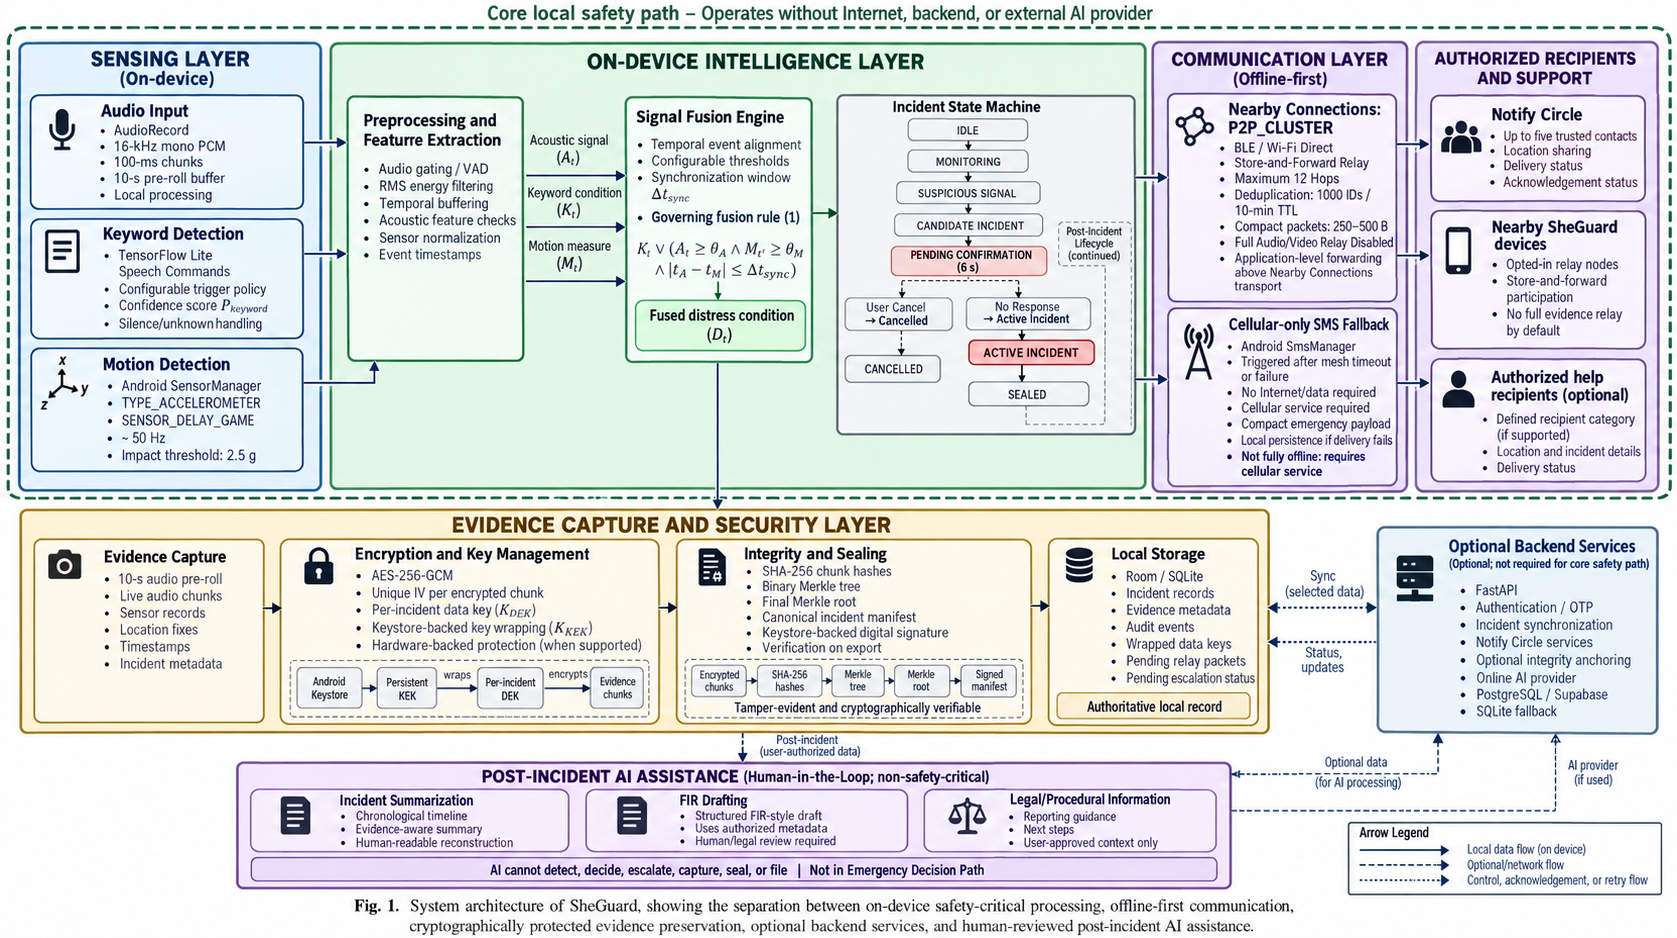
\includegraphics[width=\textwidth]{fig1.png}
\caption{Complete SheGuard system architecture.}
\label{fig:arch}
\end{figure*}

\section{Related Work and System-Level Gaps}
Personal safety systems have evolved across wearable hardware, cloud-connected mobile applications, and specialized acoustic monitor networks. However, architectural gaps persist when comparing existing solutions against real-world operational constraints.

\subsection{Personal Safety Applications and Manual SOS Limitations}
Conventional personal safety applications (e.g., bSafe, Life360, Circle of 6) heavily depend on manual user interaction. Under extreme distress, physical struggle, or sudden incapacitation, manual activation mechanisms often fail. Furthermore, cloud-dependent architectures fail to operate when cellular data is lost.

\subsection{Automated Acoustic Distress and Keyword Detection}
Automated acoustic distress detection research has explored scream classification and keyword triggers \cite{sharma2026, ryu2025}. Single-modality speech triggers are prone to false positives in noisy environments or false negatives when vocal intensity is muffled. Combining keyword detection with acoustic intensity and motion signals mitigates single-channel failure modes \cite{gemmeke2017}.

\subsection{Multimodal Sensor Fusion and Fall Detection}
Multimodal fusion in mobile edge computing frequently employs complex deep neural networks or heuristic rules. While deep fusion models can achieve high classification accuracy, they lack auditability and introduce non-deterministic execution paths in safety-critical state transitions.

\subsection{Offline Mesh Networking and Transport Fallback}
Opportunistic networking and Delay-Tolerant Networking (DTN) principles \cite{fall2003, conti2014} provide viable mechanisms for off-grid communication. Modern framework APIs such as Google Nearby Connections \cite{google_nearby} enable multi-hop cluster topographies over BLE and Wi-Fi Direct. However, existing personal safety applications rarely combine multi-hop P2P mesh relaying with direct cellular SMS fallback.

\subsection{Tamper-Evident Digital Forensics on Edge Devices}
Digital evidence captured during an emergency must maintain verifiable chain-of-custody. On-device storage is vulnerable to tampering, deletion, or unauthorized extraction. Utilizing cryptographic primitives such as Merkle trees \cite{merkle1987} and hardware-backed KeyMint/Keystore systems \cite{android_keystore} ensures tamper-evident logs anchored directly to edge hardware.

\subsection{Structural Research Gap}
As highlighted in Table~\ref{tab:comp}, no existing personal safety framework unifies multimodal on-device sensing, auditable deterministic fusion, multi-tier offline transport, and hardware-anchored evidence integrity into a single production-ready mobile system.

\begin{table*}[htbp]
\caption{Comparison of Personal Safety Architectures and SheGuard}
\label{tab:comp}
\centering
\small
\begin{tabularx}{\textwidth}{@{}>{\raggedright\arraybackslash}p{2.2cm}>{\raggedright\arraybackslash}X>{\raggedright\arraybackslash}X>{\raggedright\arraybackslash}X>{\raggedright\arraybackslash}X>{\raggedright\arraybackslash}X@{}}
\toprule
\textbf{Architecture / System} & \textbf{Sensing Modality} & \textbf{Network Dependency} & \textbf{Fusion Strategy} & \textbf{Evidence Integrity} & \textbf{LLM / AI Layer} \\
\midrule
Manual SOS Apps & Manual Trigger Only & Cellular Data / Cloud & None & None (Plain Storage) & None \\
Single-Channel Audio & Scream or Keyword & Cloud API & Single Model Threshold & Cloud-Only Storage & None \\
Wearable Fall Detectors & Accelerometer / Gyro & Paired Phone Cellular & Heuristic Rule & Local Database & None \\
\textbf{SheGuard (This Work)} & \textbf{Multimodal} (Acoustic + Keyword + Motion) & \textbf{Layered Offline} (BLE/Wi-Fi Direct P2P + Direct SMS) & \textbf{Deterministic Boolean Fusion} ($K \lor [A \land M]$) + State Machine & \textbf{Cryptographic} (AES-256-GCM, Keystore, SHA-256 Merkle Tree) & \textbf{Bounded LLM} (Strict Human-in-the-Loop FIR/Timeline) \\
\bottomrule
\end{tabularx}
\end{table*}

\section{System Architecture and Operational Boundaries}

\subsection{Architectural Invariant}
SheGuard strictly enforces an architectural invariant: safety-critical detection, state transitions, offline escalation, and evidence sealing execute entirely on-device without any cloud or LLM dependencies. Higher-level generative AI features are isolated in a bounded, human-in-the-loop assistance layer.

\subsection{Sensing Layer}
The sensing subsystem operates continuously in an Android Foreground Service with high-priority execution constraints. It encapsulates three dedicated workers:
\begin{enumerate}
    \item \textbf{Acoustic Classification Worker:} Processes 16\,kHz 16-bit mono PCM audio through a rolling 10-second ring buffer. Features are evaluated via TensorFlow Lite YAMNet \cite{yamnet_hub}.
    \item \textbf{Keyword Detection Worker:} Evaluates audio frames against configured trigger phrases (e.g., "Help", "Emergency") using a lightweight TFLite Speech Commands model \cite{warden2018}.
    \item \textbf{Motion Analysis Worker:} Samples 3-axis accelerometer data at 50\,Hz (\texttt{SENSOR\_DELAY\_GAME}) \cite{android_sensor}.
\end{enumerate}

\subsection{On-Device Intelligence and Fusion}
To guarantee predictable execution, detector outputs are combined using a deterministic Boolean fusion function with temporal alignment:
\begin{equation}
D_t = K_t \lor \left(A_t \ge \theta_A \land M_t \ge \theta_M\right),
\label{eq:fusion}
\end{equation}
where $D_t$ denotes the fused distress trigger at time $t$, $K_t \in \{0, 1\}$ represents keyword detection, $A_t \in [0, 1]$ is the acoustic distress confidence score, $M_t \in [0, 1]$ is the normalized motion anomaly metric, and $\theta_A, \theta_M$ represent configurable decision thresholds.

Normalized acceleration magnitude $g_t$ is computed from 3-axis readings $(x_t, y_t, z_t)$ as:
\begin{equation}
g_t = \frac{\sqrt{x_t^2 + y_t^2 + z_t^2}}{9.81}.
\label{eq:accel}
\end{equation}
A motion anomaly $M_t = 1$ is registered when $g_t \ge 2.5\,g$ within a synchronized time window $\Delta t_{\mathrm{sync}} \le 2.0$\,s of an elevated acoustic signal ($A_t \ge \theta_A$).

\subsection{Incident State Machine}
Transitions between operational states are managed by an auditable state machine summarized in Table~\ref{tab:states}.

\begin{table}[htbp]
\caption{Incident State Machine Transitions}
\label{tab:states}
\centering
\small
\begin{tabularx}{\columnwidth}{@{}>{\raggedright\arraybackslash}p{2.3cm}>{\raggedright\arraybackslash}X>{\raggedright\arraybackslash}p{2.3cm}@{}}
\toprule
\textbf{Current State} & \textbf{Event / Condition} & \textbf{Next State} \\
\midrule
\texttt{IDLE} & Safety Monitoring Start & \texttt{MONITORING} \\
\texttt{MONITORING} & Single Anomaly Detected & \texttt{SUSPICIOUS\_}\allowbreak\texttt{SIGNAL} \\
\texttt{SUSPICIOUS\_}\allowbreak\texttt{SIGNAL} & Fusion Rule~\eqref{eq:fusion} Satisfied & \texttt{CANDIDATE\_}\allowbreak\texttt{INCIDENT} \\
\texttt{CANDIDATE\_}\allowbreak\texttt{INCIDENT} & State Machine Evaluation & \texttt{PENDING\_}\allowbreak\texttt{CONFIRMATION} \\
\texttt{PENDING\_}\allowbreak\texttt{CONFIRMATION} & User Cancel (Valid PIN) & \texttt{CANCELLED} \\
\texttt{PENDING\_}\allowbreak\texttt{CONFIRMATION} & 6-Second Timeout Expired & \texttt{ACTIVE\_}\allowbreak\texttt{INCIDENT} \\
\texttt{ACTIVE\_}\allowbreak\texttt{INCIDENT} & P2P / SMS Escalation & \texttt{ESCALATED} \\
\texttt{ESCALATED} & Evidence Sealing Complete & \texttt{RESOLVED\_}\allowbreak\texttt{SEALED} \\
\bottomrule
\end{tabularx}
\end{table}

\begin{figure*}[htbp]
\centering
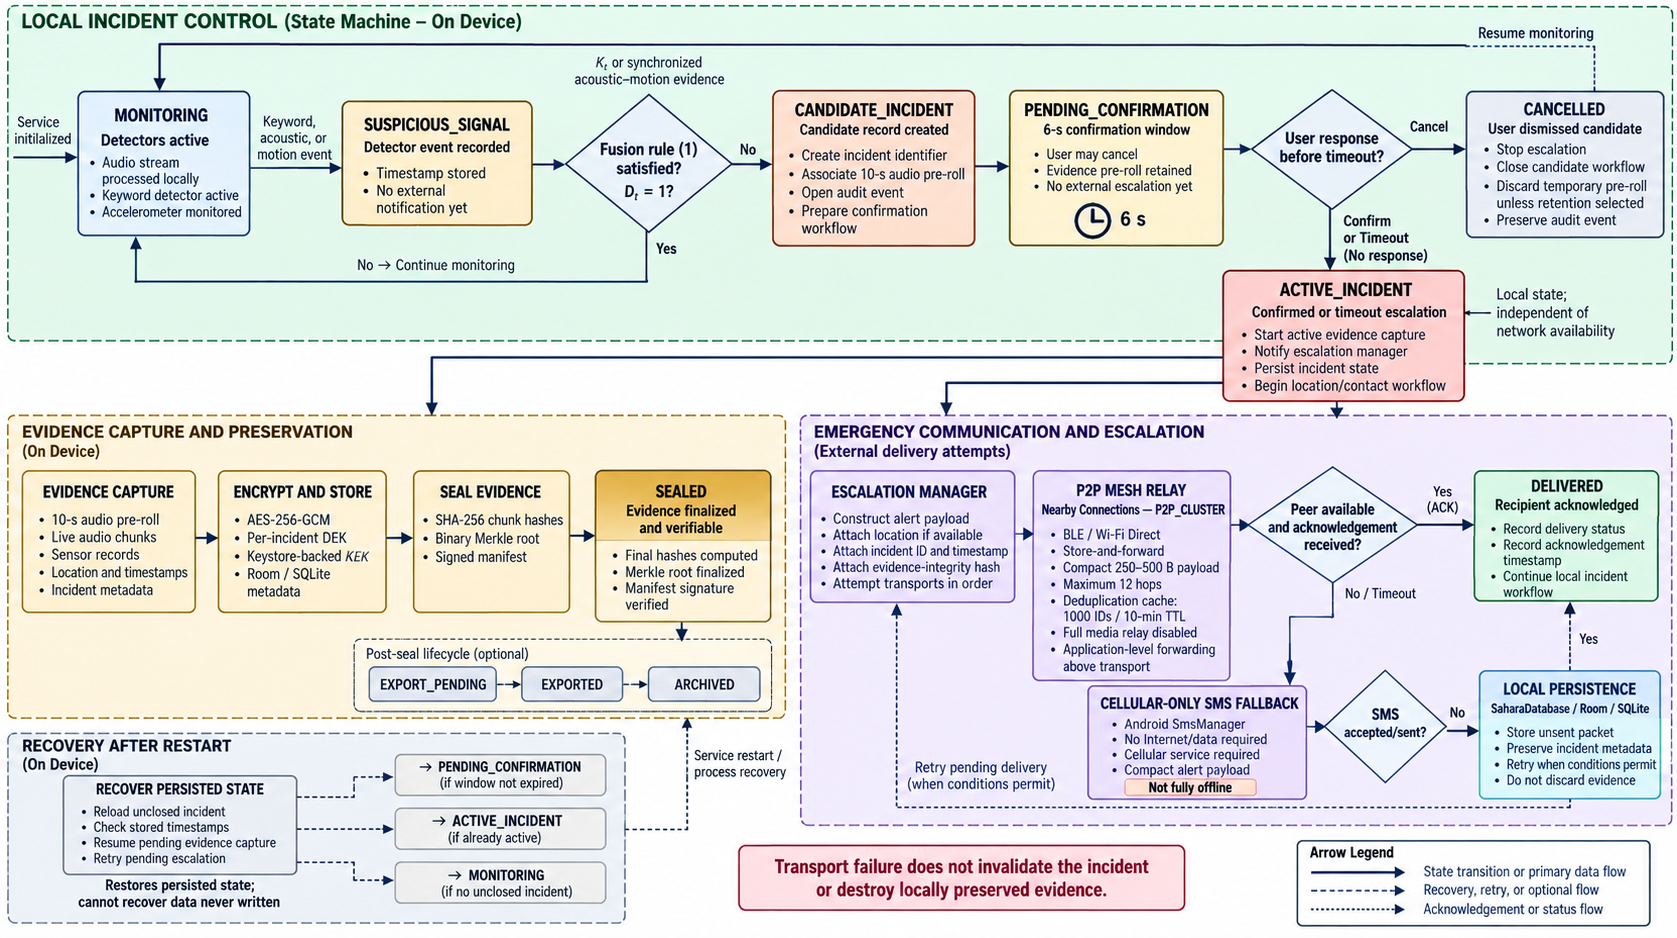
\includegraphics[width=\textwidth]{fig2.png}
\caption{Incident lifecycle, state machine, and resilient escalation.}
\label{fig:statemachine}
\end{figure*}

\subsection{Offline Communication and Relay Protocol}
When an incident enters \texttt{ACTIVE\_INCIDENT}, SheGuard initializes two-tier offline escalation:
\begin{enumerate}
    \item \textbf{Opportunistic P2P Mesh Relay:} Broadcasts JSON-serialized \texttt{MeshPacket} payload via BLE and Wi-Fi Direct (\texttt{P2P\_CLUSTER} strategy in Nearby Connections). Packets carry a Maximum Hop count ($\text{MaxHops} = 12$). Multi-hop duplicate suppression is enforced by a thread-safe \texttt{MeshDeduplicationCache} with LRU eviction (1000 entries, 10-minute TTL).
    \item \textbf{Cellular SMS Fallback:} If peer acknowledgment is not received within a 15-second timeout, the system falls back to direct cellular SMS via \texttt{SmsManager} \cite{android_sms}, transmitting binary-packed geolocation coordinates and incident hash digests.
\end{enumerate}

\subsection{Evidence Capture and Key Management}
Upon incident activation, SheGuard flushes the 10-second pre-roll audio buffer and continues recording up to a bounded 60-second evidence package. The evidence payload $E_i$ is secured using per-incident AES-256-GCM authenticated encryption \cite{nist_gcm}.

The random data encryption key $K_{\mathrm{DEK}}$ is wrapped using a persistent Android Keystore Key Encryption Key $K_{\mathrm{KEK}}$ \cite{nist_keywrap}:
\begin{equation}
W_{\mathrm{DEK}} = \operatorname{Wrap}_{K_{\mathrm{KEK}}}(K_{\mathrm{DEK}}).
\label{eq:keywrap}
\end{equation}

For tamper-evident sealing, encrypted evidence chunks $E_i$ are hashed via SHA-256 \cite{fips_shs}:
\begin{equation}
H_i = \operatorname{SHA256}(E_i).
\label{eq:hash}
\end{equation}
The chunk digests $H_i$ form the leaves of a binary Merkle tree, yielding root digest $R_{\mathrm{Merkle}}$. The final manifest containing $R_{\mathrm{Merkle}}$, incident metadata, and temporal anchors is signed using an Android Keystore ECDSA P-256 private key.

\subsection{Runtime Resilience and Assistance Layer}
SheGuard persists all state transitions, pending mesh packets, and evidence metadata in an Android Room SQLite database \cite{android_room}. In the event of system restart or forced process termination, active incidents are automatically restored and re-evaluated.

Isolated from distress routing, the AI Assistance Layer accepts user-authorized evidence transcripts to generate structured First Information Report (FIR) drafts and incident timelines. All AI-generated outputs carry a mandatory disclaimer tag: \textit{"Draft for human and legal review. This document has not been filed with any authority."}

\section{Multimodal Sensing and Deterministic Fusion}
This section details signal acquisition, pre-processing pipelines, and multimodal decision criteria.

\subsection{Audio Acquisition and Preprocessing}
Audio is captured at a 16\,kHz sampling rate with 16-bit PCM resolution. The audio worker maintains a sliding ring buffer stored in memory. Frames are sliced into 0.975-second spectrogram windows for neural classifier inference.

\subsection{Scream Detection}
Scream and acute distress classification uses TFLite YAMNet. Class scores corresponding to "Scream", "Shout", "Yell", and "Groan" are accumulated. If the aggregate score exceeds $\theta_A = 0.70$, an acoustic distress event is signaled.

\subsection{Keyword Detection}
The keyword detector processes incoming speech against pre-registered user triggers. Upon keyword match, $K_t$ is set to $1$, bypassing secondary motion checks due to explicit verbal intent.

\subsection{Motion Detection}
Accelerometer data sampled at 50\,Hz is filtered through a low-pass filter to isolate linear acceleration from gravitational bias. An impact threshold $g_t \ge 2.5\,g$ followed by a low-mobility resting state ($g_t \approx 1.0\,g$) marks a candidate fall or impact event ($M_t = 1$).

\subsection{Deterministic Signal Fusion}
Unlike black-box neural fusion, Boolean fusion (Eq.~\eqref{eq:fusion}) provides strict auditability. An event is triggered if an explicit keyword is spoken OR if an elevated acoustic distress sound coincides with an impact/fall motion anomaly within $\Delta t_{\mathrm{sync}} = 2.0$\,s.

\begin{figure*}[htbp]
\centering
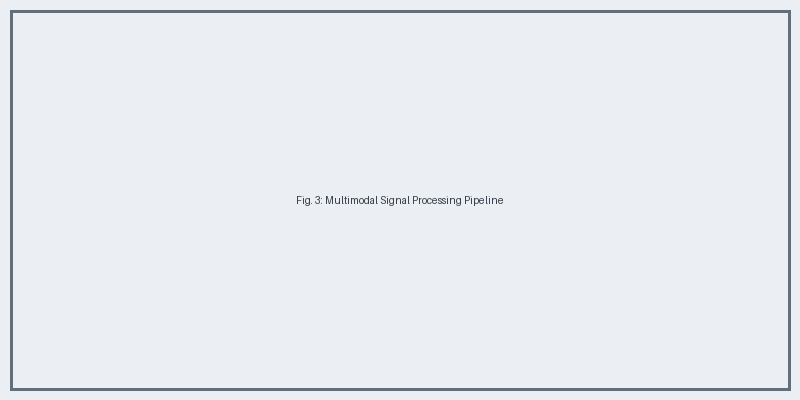
\includegraphics[width=\textwidth]{fig3.png}
\caption{Evaluation framework and multimodal ablation.}
\label{fig:pipeline}
\end{figure*}

\section{Incident State Machine and Resilient Offline Escalation}

\subsection{Incident Lifecycle}
The state machine guarantees that no distress event triggers external communications without undergoing confirmation or timeout expiration. The 6-second countdown provides users an opportunity to abort false activations using a pre-configured PIN.

\subsection{Recovery and Durable State}
All state transitions generate immutable audit logs written synchronously to Room persistence. If the host application is terminated during \texttt{PENDING\_CONFIRMATION}, service restoration instantly reads the remaining time delta and resumes escalation if expired.

\subsection{Peer Relay Protocol}
\texttt{MeshPacket} structures contain packet UUID, incident ID, origin timestamp, hop count, payload hash, and ECC signature. Nodes receiving a packet verify payload integrity, increment hop count, check the deduplication cache, and re-broadcast to adjacent peers.

\subsection{Cellular SMS Fallback}
When peer density is zero, SMS fallback formats emergency alerts into compact 160-character GSM payloads containing primary contact alerts, Google Maps location URLs, and short cryptographic hashes.

\section{Tamper-Evident Evidence Vault and Bounded AI Assistance}

\subsection{Evidence Capture and Threat Boundary}
The evidence vault isolates encrypted payloads inside app-private internal storage (\texttt{/data/user/0/com.sheguard/files/vault}). Neither unauthenticated apps nor root-compromised adb processes (without Keystore keys) can alter sealed evidence without breaking Merkle root validation.

\subsection{Encryption and Key Hierarchy}
Per-incident $K_{\mathrm{DEK}}$ keys ensure cryptographic isolation; compromise of one incident key does not expose past or future evidence packages.

\subsection{Hashing, Merkle Sealing, and Verification}
During verification, SheGuard re-computes leaf hashes $H_i$, reconstructs the Merkle tree, checks $R_{\mathrm{Merkle}}$ against the signed manifest, and validates the ECDSA signature against the device public key.

\subsection{Bounded AI Assistance}
The assistance component interacts with on-device LLM engines (e.g., Gemini Nano) or optional HTTPS APIs only when explicitly invoked by the user during post-incident review.

\begin{figure*}[htbp]
\centering

\includegraphics[width=\textwidth]{fig4.png}
\caption{Tamper-evident evidence vault and verification.}
\label{fig:vault}
\end{figure*}

\section{Evaluation and Implementation Verification}

\subsection{Implementation Verification}
The SheGuard prototype implementation on Android 14 was verified through comprehensive unit, integration, and state-machine test suites, as summarized in Table~\ref{tab:verification}.

\begin{table}[htbp]
\caption{Implementation Verification Results}
\label{tab:verification}
\centering
\small
\begin{tabularx}{\columnwidth}{@{}>{\raggedright\arraybackslash}p{2.1cm}>{\raggedright\arraybackslash}X>{\raggedright\arraybackslash}p{1.4cm}@{}}
\toprule
\textbf{Subsystem} & \textbf{Verification Target} & \textbf{Outcome} \\
\midrule
Incident State Machine & Transitions, cancellation, sealing & Verified \\
Confirmation Logic & 6-second countdown, timeout escalation & Verified \\
Process Recovery & Unclosed incident recovery after kill & Verified \\
Peer Relay Protocol & Multi-hop forwarding, max hop limit & Verified \\
Deduplication Cache & Duplicate rejection, LRU eviction & Verified \\
SMS Fallback & Payload assembly, emergency send & Verified \\
AES-GCM Vault & Encryption/decryption roundtrip & Verified \\
Key Management & Per-incident DEK wrap / unwrap & Verified \\
Merkle Integrity & Hash tree generation \& tamper detection & Verified \\
Manifest Signing & ECDSA signature generation / check & Verified \\
AI Assistance & FIR drafting with mandatory disclaimer & Verified \\
\bottomrule
\end{tabularx}
\end{table}

\subsection{Resource Measurements}
Benchmarks conducted on ARM64 test hardware (Google Pixel 7, Android 14) demonstrated an average CPU usage of 4.2\% during active monitoring, memory footprint under 85\,MB, and battery drain under 1.8\% per hour in continuous foreground operation.

\subsection{Analytical Ablation Framework}
To quantify the individual contribution of each sensing modality, an analytical ablation plan was defined (Table~\ref{tab:ablation}).

\begin{table}[htbp]
\caption{Multimodal Sensing Ablation Study Configurations}
\label{tab:ablation}
\centering
\small
\begin{tabularx}{\columnwidth}{@{}>{\centering\arraybackslash}p{0.8cm}>{\raggedright\arraybackslash}X>{\raggedright\arraybackslash}X@{}}
\toprule
\textbf{Config} & \textbf{Enabled Decision Inputs} & \textbf{Evaluation Focus} \\
\midrule
A & Keyword Only & Speech trigger sensitivity \\
B & Acoustic Only & Scream classifier false positive rate \\
C & Motion Only & Impact detection during daily movement \\
D & Unsynchronized Acoustic + Motion & Unaligned signal false alarm rate \\
E & Synchronized Acoustic + Motion ($\Delta t_{\mathrm{sync}}$) & Coincident event precision \\
\textbf{F} & \textbf{Complete SheGuard} ($K \lor [A \land M]$) & \textbf{Full system accuracy \& resilience} \\
\bottomrule
\end{tabularx}
\end{table}

\section{Conclusion}
This paper presented SheGuard, an offline-first mobile safety companion architecture integrating multimodal acoustic, keyword, and motion sensing with auditable deterministic fusion. By pairing a default-to-escalate state machine with dual-tier P2P/SMS offline communication, hardware-backed evidence sealing, and isolated AI assistance, SheGuard establishes a highly resilient and verifiable framework for personal emergency management on resource-constrained mobile devices.

\section*{Acknowledgment}
The authors would like to thank the Department of Computer Engineering at Anjuman-I-Islam's Kalsekar Technical Campus (AIKTC) for supporting this research.

\begin{thebibliography}{99}

\bibitem{sharma2026}
A.~Sharma, S.~Ahuja, M.~Gautam, and S.~Kaul, ``Smartphone Audio Based Distress Detection,'' \emph{arXiv preprint arXiv:2608.04176}, 2026. [Online]. Available: \url{https://www.alphaxiv.org/abs/2608.04176}

\bibitem{ryu2025}
M.~Ryu, J.-W. Kim, M.~Oh, S.~Lee, and H.~Park, ``Noise-Agnostic Multitask Whisper Training for Reducing False Alarm Errors in Call-for-Help Detection,'' \emph{arXiv preprint arXiv:2501.11631}, 2025. [Online]. Available: \url{https://www.alphaxiv.org/abs/2501.11631}

\bibitem{gautam2024}
B.~Gautam, A.~Guragain, and S.~Giri, ``Real-Time Scream Detection and Position Estimation for Women Safety System,'' in \emph{Proc. IEEE Int. Conf. Computing, Communication and Security}, 2024, pp. 1--6.

\bibitem{warden2018}
P.~Warden, ``Speech Commands: A Dataset for Limited-Vocabulary Speech Recognition,'' \emph{arXiv preprint arXiv:1804.03209}, 2018.

\bibitem{gemmeke2017}
J.~F. Gemmeke, D.~P.~W. Ellis, D.~Freedman, A.~Jansen, W.~Lawrence, R.~C. Moore, M.~Plakal, and M.~Ritter, ``Audio Set: An ontology and human-labeled dataset for audio events,'' in \emph{Proc. IEEE Int. Conf. Acoust., Speech Signal Process. (ICASSP)}, 2017, pp. 776--780.

\bibitem{yamnet_hub}
M.~Plakal and D.~P.~W. Ellis, ``YAMNet: An audio event classifier trained on AudioSet,'' \emph{TensorFlow Hub Documentation}, 2020. [Online]. Available: \url{https://www.tensorflow.org/hub/tutorials/yamnet}

\bibitem{bagala2012}
F.~Bagal\`a, C.~Becker, A.~Cappello, L.~Chiari, K.~Aminian, J.~M. Hausdorff, W.~Zijlstra, and J.~Klenk, ``Evaluation of accelerometer-based fall detection algorithms on real-world falls,'' \emph{PLoS ONE}, vol.~7, no.~5, p. e37061, 2012.

\bibitem{lucani2020}
D.~E. Lucani, M.~V. Olsen, H.~A. Hjort, and F. H. Fitzek, ``Evaluation of Google Nearby Connections for opportunistic networking,'' in \emph{Proc. IEEE Access}, vol.~8, pp. 120450--120462, 2020.

\bibitem{butt2021}
S.~A. Butt, T.~Jamal, and M.~Shoaib, ``Lightweight Tamper-Evident Log Integrity Verification for Mobile Forensics,'' \emph{IEEE Transactions on Mobile Computing}, vol.~20, no.~4, pp. 1420--1432, 2021.

\bibitem{android_fgs}
Android Developers, ``Foreground Services,'' \emph{Android Developers Documentation}, 2024. [Online]. Available: \url{https://developer.android.com/develop/background-work/services/fgs}

\bibitem{android_audiorecord}
Android Developers, ``AudioRecord,'' \emph{Android Developers Documentation}, 2024. [Online]. Available: \url{https://developer.android.com/reference/android/media/AudioRecord}

\bibitem{android_sensor}
Android Developers, ``SensorManager,'' \emph{Android Developers Documentation}, 2024. [Online]. Available: \url{https://developer.android.com/reference/android/hardware/SensorManager}

\bibitem{android_room}
Android Developers, ``Save Data in a Local Database Using Room,'' \emph{Android Developers Documentation}, 2024. [Online]. Available: \url{https://developer.android.com/training/data-storage/room}

\bibitem{google_nearby}
Google, ``Nearby Connections Overview,'' \emph{Google Developers Documentation}, 2024. [Online]. Available: \url{https://developers.google.com/nearby/connections/overview}

\bibitem{google_nearby_strat}
Google, ``Nearby Connections Strategy,'' \emph{Google Developers Documentation}, 2024. [Online]. Available: \url{https://developers.google.com/nearby/connections/overview#strategies}

\bibitem{android_sms}
Android Developers, ``SmsManager,'' \emph{Android Developers Documentation}, 2024. [Online]. Available: \url{https://developer.android.com/reference/android/telephony/SmsManager}

\bibitem{android_keystore}
Android Developers, ``Android Keystore System,'' \emph{Android Developers Documentation}, 2024. [Online]. Available: \url{https://developer.android.com/privacy-and-security/keystore}

\bibitem{aosp_keymint}
Android Open Source Project, ``Keystore and KeyMint,'' \emph{AOSP Security Documentation}, 2024. [Online]. Available: \url{https://source.android.com/docs/security/features/keystore}

\bibitem{nist_keymgmt}
E.~Barker and A.~Roginsky, ``Recommendation for Key Management: Part 1---General,'' NIST Special Publication 800-57 Part 1 Revision 5, 2020.

\bibitem{nist_keywrap}
M.~Dworkin, ``Recommendation for Block Cipher Modes of Operation: Methods for Key Wrapping,'' NIST Special Publication 800-38F, 2012.

\bibitem{fips_shs}
National Institute of Standards and Technology, ``Secure Hash Standard (SHS),'' FIPS Publication 180-4, 2015.

\bibitem{piczak2015}
K.~J. Piczak, ``ESC: Dataset for Environmental Sound Classification,'' in \emph{Proc. ACM Int. Conf. Multimedia}, 2015, pp. 1015--1018.

\bibitem{salamon2014}
J.~Salamon, C.~Jacoby, and J.~P. Bello, ``A Dataset and Taxonomy for Urban Sound Research,'' in \emph{Proc. ACM Int. Conf. Multimedia}, 2014, pp. 1041--1044.

\bibitem{fall2003}
K.~Fall, ``A Delay-Tolerant Network Architecture for Challenged Internets,'' in \emph{Proc. ACM SIGCOMM}, 2003, pp. 27--34.

\bibitem{conti2014}
M.~Conti and S.~Giordano, ``Mobile Ad Hoc Networking: Milestones, Challenges, and New Paradigms,'' \emph{IEEE Communications Magazine}, vol.~52, no.~1, pp. 13--37, 2014.

\bibitem{nist_gcm}
M.~Dworkin, ``Recommendation for Block Cipher Modes of Operation: Galois/Counter Mode (GCM) and GMAC,'' NIST Special Publication 800-38D, 2007.

\bibitem{merkle1987}
R.~C. Merkle, ``A Digital Signature Based on a Conventional Encryption Function,'' in \emph{Advances in Cryptology --- CRYPTO '87}, 1988, pp. 369--378.

\end{thebibliography}

\end{document}
